\documentclass[a4paper,12pt]{article}
\usepackage{array}
\usepackage[utf8]{inputenc}
\usepackage[spanish]{babel}
\usepackage{graphicx}
\usepackage{tabulary}
\usepackage{tabularx}
\usepackage{slashbox}
\usepackage{rotating}

% control de márgenes
\usepackage{anysize} 
% Controla los márgenes {izquierda}{derecha}{arriba}{abajo}.
\marginsize{3cm}{2cm}{2cm}{2cm}



% cabecera y pie
\usepackage{fancyhdr} % activamos el paquete
\pagestyle{fancy} % seleccionamos un estilo
\lhead{Seminario de Sistemas Embebidos - FiUBA} % texto izquierda de la cabecera
\chead{} % texto centro de la cabecera
\rhead{Capear} 
\lfoot{Bos - Petrella} % texto izquierda del pie
\cfoot{} 
\rfoot{pág. \thepage} % texto derecha del pie
\renewcommand{\headrulewidth}{0.4pt} % grosor de la línea de la cabecera
\renewcommand{\footrulewidth}{0.4pt} % grosor de la línea del pie


\begin{document}

\thispagestyle{empty}

\begin{center}
	
\includegraphics[width=0.2\textwidth,angle=0]{./imagenes/logo-facu.png}\\
	\huge{{Universidad de Buenos Aires}}\\
	\huge{{Facultad de Ingeniería}}\\
	\vspace{2.2cm}
	\Huge{\textbf{Seminario de Sistemas Embebidos}}\\
	\vspace{0.5cm}
	\Large{\textbf{Cortacorriente para Equipo Autónomo de Red}}\\
	\vspace{1.5cm}
	\Large{$2^{do}$ cuatrimestre de 2012}\\
	\vspace{2cm}	
\end{center}

\vfill
\begin{flushright}
		\textbf{Alumnos:}  Matías Petrella (68405)\\
		 Patricio Bos (81163)\\
		\textbf{Fecha:}  22/02/13\\
\end{flushright}
\newpage



\tableofcontents
\thispagestyle{empty}
\newpage

%------------------------------------------------------------------------------------------------
%------------------------------------------------------------------------------------------------
\section{Introducción}
%------------------------------------------------------------------------------------------------
%------------------------------------------------------------------------------------------------
Problema inherente a los dispositivos autónomos de red\\
 
Los equipos de red ``autónomos'' --es decir, aquellos que en condiciones normales de trabajo no interactúan con humanos, tales como: switches, routers, camaras IP, servidores no asistidos, almacenamiento RAID directo a red, puntos de acceso inalámbricos, etc.-- son susceptibles de interrumpir su servicio en forma repentina. Normalmente la solución a este problema es tan simple como cortar el suministro de corriente durante unos segundos y luego restituirlo. Este procedimiento fuerza al equipo ``colgado'' a reiniciarse, en cuyo proceso se restablecen las variables de trabajo y (posiblemente) se realiza un autodiagnostico tras lo cual vuelven a prestar servicio en forma normal.\\

Las ventajas de disponer de un equipo igualmente autónomo que pueda detectar estas salidas de servicio y accionar sobre el suministro eléctrico son múltiples:

\begin{itemize}
\item detección temprana de fallas
\item aumento en la disponibilidad de los servicios
\item ahoro en los costos de mantenimiento 
\item posibilidad de instalación en zonas de dificil acceso
\item etc.
\end{itemize}


El LPCXpresso es un toolchain completo de desarrollo y evaluación para microcontroladores de NXP.
Se compone de los siguientes elementos:
\begin{itemize}
\item LPCXpresso IDE y herramientas de desarrollo
\item LPCXpresso target board (stick)
\item LPCXpresso Baseboard EA-XPR-021
\end{itemize}

Se propone utilizar el entorno de desarrollo LPCXpresso para implementar un {\textbf{Cortacorriente para equipos autónomos de red}}. Se pretende desarrollar una interfaz web para configurar el sistema\\ 

El proyecto se segmenta en los siguientes 10 items.

\begin{enumerate}
\item Determinar que stack de TCP/IP se va a utilizar y probarlo. (LwIP, uIP, NicheLite, etc)
\item Diseñar e implementar una API por sobre el stack para abstraerse del mismo y poder realizar los pings.
\item Diseñar e implementar la página HTML para administrar el sistema.
\item Utilizar el stack seleccionado para poner en marcha un web server y montar la página.
\item Implementar o buscar implementaciones de la funcionalidad PING y probarla.
\item Diseñar e implementar una API para poder manejar las salidas digitales y otra para el Watchdog Timer.
\item Implementar la funcionalidad para chequear paginas web por telnet y actuar en consecuencia. (ó implementación del PCB para el módulo de control)
\item Implementar una interfaz de potencia. 
\item Combinar los items anteriores para implementar el sistema, pensar en la utilización de un RTOS.
\item Entrega de Informe Final.
\end{enumerate}

$\left({\frac{x^2+15}{10 \rho}}\right)$

%------------------------------------------------------------------------------------------------
%------------------------------------------------------------------------------------------------
\newpage
\section{Desarrollo}
%------------------------------------------------------------------------------------------------
%------------------------------------------------------------------------------------------------
\subsection{PCB interfaz de potencia}
Para que el MCU pueda administrar el suministro eléctrico de los equipos autónomos de red, se implementa una interfaz de potencia 5VDC/220VAC de 4 canales.  Para tal fin se utlizan optoacopladores MOC3021 y triacs BTA12 aislados, de propositos generales.\\

La conmutación se realiza sobre el neutro de la línea de 220VAC, mientras que la carga se conecta al vivo.\\


\begin{figure}[ht]
	\begin{minipage}[b]{0.45\linewidth}
		\centering
		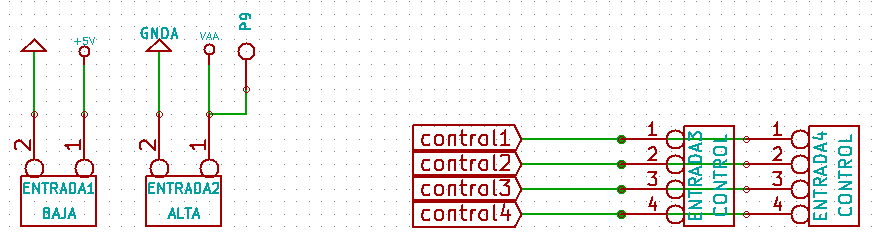
\includegraphics[width=\textwidth]{./imagenes/potencia-schema1.png}
		\caption{conectores}
		\label{fig:figure1}
	\end{minipage}
	\hspace{0.5cm}
	\begin{minipage}[b]{0.45\linewidth}
		\centering
		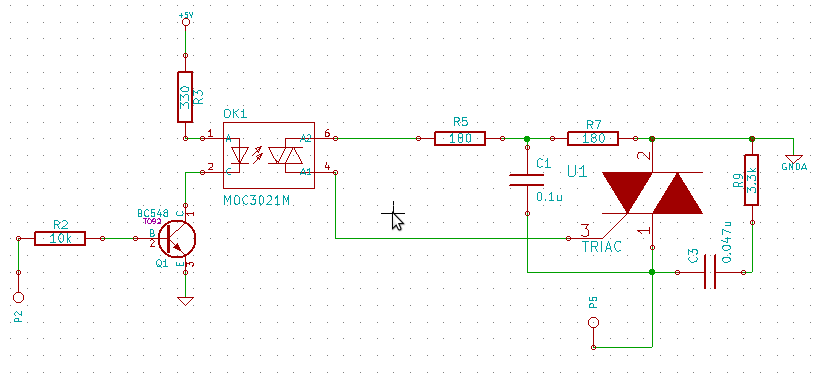
\includegraphics[width=\textwidth]{./imagenes/potencia-schema2.png}
		\caption{interfaz 5VDC/220VAC}
		\label{fig:figure2}
	\end{minipage}
\end{figure}

Al desconocerse el tipo de carga que será conectada deben tomarse precausiones para proteger el triac y el optoacoplador. Se utilizan dos redes snubber compuestas por un capacitor de $0.047\mu F$ y un resistor de $3.3k\Omega$ para el triac y un capacitor de $0.1\mu F$ y un resistor de $180\Omega$ para el optoacoplador.\\

Para aislar la excitación del optoacoplador de la capacidad de suministro de corrientes del MCU, la misma se realiza con un transistor bipolar NPN BC548.\\

\begin{figure}[ht]
	\begin{minipage}[b]{0.45\linewidth}
		\centering
		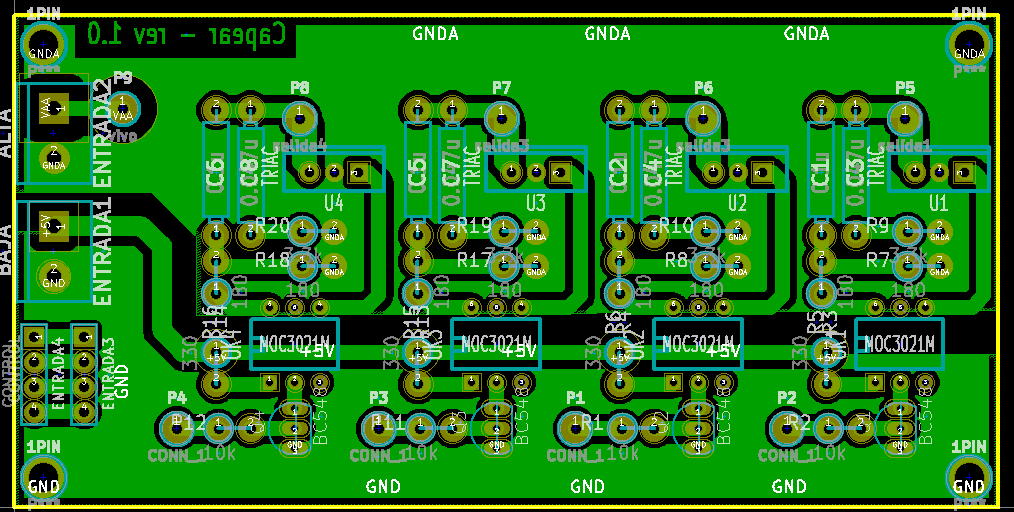
\includegraphics[width=\textwidth]{./imagenes/potencia-PCB.png}
		\caption{PCB layout}
		\label{fig:figure3}
	\end{minipage}
	\hspace{0.5cm}
	\begin{minipage}[b]{0.45\linewidth}
		\centering
		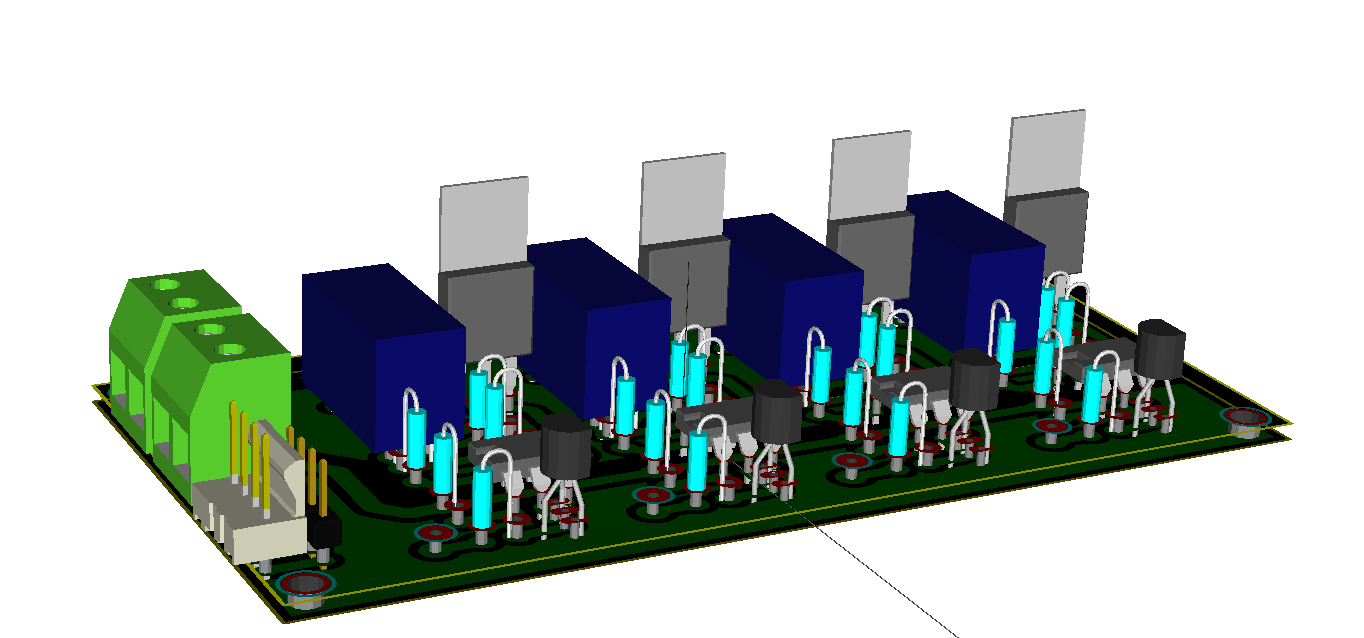
\includegraphics[width=\textwidth]{./imagenes/potencia-3D.png}
		\caption{vista 3D}
		\label{fig:figure4}
	\end{minipage}
\end{figure}


\section{algo}
\section{Conclusiones}
Se pudo desarrollar un sistema que cumpla con todos los objetivos propuestos haciendo uso extensivo de las funciones propias del {\textit{port}} de freeRTOS para LPC1769, así como también de la librería CMSIS provista por NXP.\\
Se utilizaron funciones ISRsafe dentro de las rutinas de interrupción y se forzó el llamado al schedule al finalizar las mismas para asegurar el cambio de contexto como práctica de buena programación.
En cuanto a la elección de las prioridades, se optó por asignar prioridades distintas a cada tarea. La mas baja a la tarea periódica y la mayor a la tarea asociada al RTC.  No obstante lo cual, todas las tareas hacen uso de la UART cuya disponibilidad esta restringida a un mutex.  Por este motivo ninguna tarea es {\textit{pre-empted}} ya que tomar el mutex le asegura permanecer en estado running.


\end{document}